
In this chapter, we present the evaluation results for JOP. In the
following section, the hardware platform that is used for
benchmarking is described. This is followed by a comparison of JOP's
resource usage with other soft-core processors. In
Section~\ref{sec:performance} the performance of a number of
different solutions for embedded Java is compared with embedded
application benchmarks. Comparison at bytecode level can be found in
\cite{jop:austrochip05}. This chapter concludes with a description of
real-world applications based on JOP.

\section{Hardware Platforms}

During the development of JOP and its predecessors, several
different FPGA boards were developed. The first experiments involved
using Altera FPGAs EPF8282,\linebreak[4] EPF8452, EPF10K10 and ACEX
1K30 on boards that were connected to the printer port of a PC for
configuration, download and communication. The next step was the
development of a stand-alone board with FLASH memory and static RAM.
This board was developed in two variants, one with an ACEX 1K50 and
the other with a Cyclone EP1C6 or EP1C12. Both boards are
pin-compatible and are used in commercial applications of JOP. The
Cyclone board is the hardware that is used for the following
evaluations.

This board is an ideal development platform for JOP. Static RAM and
FLASH are connected via independent buses to the FPGA. All unused
FPGA pins and the serial line are available via four connectors. The
FLASH can be used to store configuration data for the FPGA and
application program/data. The FPGA can be configured with a
ByteBlasterMV download cable or loaded from the FLASH (with a small
CPLD on board). As the FLASH is also connected to the FPGA, it can be
programmed from the FPGA. This allows for upgrades of the Java
program and even the processor core itself in the field. The board is
slightly different from other FPGA prototyping boards, in that its
connectors are on the bottom side. Therefore, it can be used as a
module (60~mm x 48~mm), i.e.\ as part of a larger board that contains
the periphery. The Cyclone board contains:
%
%\begin{samepage}
\begin{itemize}
\item Altera Cyclone EP1C6Q240 or EP1C12Q240
\item Step Down voltage regulator (1V5)
\item Crystal clock (20~MHz) at the PLL input (up to 640~MHz
    internal)
\item 512~KB FLASH (for FPGA configuration and program code)
\item 1~MB fast asynchronous RAM (15 ns)
\item Up to 128~MB NAND FLASH
\item ByteBlasterMV port
\item Watchdog with a LED
\item EPM7064 PLD to configure the FPGA from the FLASH on watchdog reset
\item Serial interface driver (MAX3232)
\item 56 general-purpose I/O pins
\end{itemize}
%\end{samepage}
%
The RAM consists of two independent 16-bit banks (with their own
address and control lines). Both RAM chips are on the bottom side of
the PCB, directly under the FPGA pins. As the traces are very short
(under 10~mm), it is possible to use the RAMs at full speed without
reflection problems. The two banks can be combined to form 32-bit
RAM or support two independent CPU cores. Pictures and the schematic
of the board can be found in Appendix~\ref{appx:cycore}.

\index{Baseio}

The expansion board Baseio hosts the CPU module and provides a
complete Java processor system with Internet connection. A step down
switching regulator with a large AC/DC input range supplies the core
board. All input and output pins are EMC/ESD-protected and routed to
large connectors (5.08~mm Phoenix). Analog comparators can be used to
build sigma-delta ADCs. For FPGA projects with a network connection,
a CS8900 Ethernet controller with an RJ45 connector is included on
the expansion board. Pictures and the schematic of the board can be
found in Appendix~\ref{appx:baseio}.


\section{Chip Area and Clock Frequency}

Cost is an important issue for embedded systems. The cost of a chip
is directly related to the die size (the cost per die is roughly
proportional to the square of the die area \cite{Hennessy02}).
Processors for embedded systems are therefore optimized for minimum
chip size. In this section, we will compare JOP with different
processors in terms of size. One major design objective in the
development of JOP was to create a small system that can be
implemented in a low-cost FPGA.


Table~\ref{tab:soft-cores} compares the resource consumption and
maximum clock frequency of a time-predictable processor (JOP), a
standard MIPS architecture (YARI), the LEON SPARC processor, and a
complex Java processor (picoJava), when implemented in the same FPGA
(Altera EP1C6/12 FPGA \cite{AltCyc}). For the resource comparison we
compare the consumption of the two basic structures of an FPGA; Logic
cells (LC) and embedded memory blocks. The maximum frequency for all
soft-core processors is in the same technology.

\index{Java processor!picoJava}

\begin{table}
  \begin{center}
    \begin{tabular}[t]{lrrr}
        \toprule
      Soft-core    & Logic Cells & Memory  & Frequency \\
        \midrule
      JOP          & 3,300       &  7.6 KB & 100~MHz    \\
      YARI         & 6,668       & 18.9 KB & 75~MHz     \\
      LEON3        & 7,978       & 10.9 KB & 35~MHz \\
      picoJava     & 27,560      & 47.6 KB & 40~MHz     \\
        \bottomrule
    \end{tabular}
  \end{center}
    \caption{Resource consumption and maximum operating frequency of JOP, YARI, LEON3, and picoJava.}
    \label{tab:soft-cores}
\end{table}

%        Lightfoot\footnotemark \cite{Lightfoot} & 3400 & 4 & 40 \\
%        NIOS A \cite{NIOS} & 1828 & 6.2 & 120 \\
%        NIOS B \cite{NIOS} & 2923 & 5.5 & 119 \\
%        SPEAR\footnotemark \cite{Delvai:ECRTS2003} & 1700 & 8 & 80 \\

JOP is configured with a 1~KB stack cache, 2~KB microcode ROM, and
4~KB method cache with 16 blocks. YARI is a MIPS compatible soft-core
\cite{cacao:yari:techrep}, optimized for FPGA technology. YARI is
configured with a 4-way set-associative instruction cache and a 4-way
set-associative write-through data cache. Both caches are 8~KB. LEON3
\cite{LEON}, the open-source implementation of the SPARC V8
architecture, has been ported to the exact same hardware that was
used for the JOP numbers. LEON3 is representative for a RISC
processor that is used in embedded real-time systems (e.g., by ESA
for space missions). The size a frequency numbers of picoJava-II
\cite{pJ1} are taken from an implementation in a Altera Cyclone-II
FPGA \cite{master:puffitsch}.



The streamlined architecture of JOP results in a small design: JOP is
half the size of the MIPS core YARI or the SPARC core LEON. Compared
with picoJava, JOP consumes about 12\% of the resources. JOP's size
allows implementing a CMP version of JOP even in a low-cost FPGA. The
simple pipeline of JOP achieves the highest clock frequency of the
three designs. From the frequency comparison we can estimate that the
maximum clock frequency of JOP in an ASIC will also be higher than a
standard RISC pipeline in an ASIC.

%The vendor independent and open-source RISC processor LEON can be
%clocked only with 35\% of JOP's frequency.

To prove that the VHDL code for JOP is as portable as possible, JOP
was also implemented in a Xilinx Spartan-3 FPGA \cite{Spartan3}. Only
the instantiation and initialization code for the on-chip memories is
vendor-specific, whilst the rest of the VHDL code can be shared for
the different targets. JOP consumes about the same LC count in the
Spartan device, but has a slower clock frequency (83~MHz).


%All configurations of JOP contain the on-chip microcode memory, the
%1~KB stack cache, a 1~KB method cache, a memory interface to a
%32-bit static RAM, and an 8-bit FLASH interface for the Java program
%and the FPGA configuration data. The minimum configuration
%implements multiplication and the shift operations in microcode. In
%the typical configuration, these operations are implemented as a
%sequential Booth multiplier and a single-cycle barrel shifter. The
%typical configuration also contains some useful I/O devices such as
%an UART and a timer with interrupt logic for multi-threading. The
%typical configuration of JOP consumes about 30\% of the LCs in a
%Cyclone EP1C6, thus leaving enough resources free for
%application-specific logic.

%As a reference, NIOS \cite{NIOS}, Altera's popular RISC soft-core, is
%also included in \tablename~\ref{tab_results_compare}. NIOS has a
%16-bit instruction set, a 5-stage pipeline and can be configured with
%a 16 or 32-bit datapath. Version A is the minimum configuration of
%NIOS. Version B adds an external memory interface, multiplication
%support, and a timer. Version A is comparable with the minimal
%configuration of JOP, and Version B with its typical configuration.



Table~\ref{tab:results:gate:count} provides gate count estimates for
JOP, picoJava, the aJile processor, and, as a reference, an old Intel
Pentium MMX processor. Equivalent gate count for an LC\footnote{The
factors are derived from the data provided for various processors in
Chapter~\ref{chap:related} and from the resource estimates in
\cite{jop:stack}.} varies between 5.5 and 7.4 -- we chose a factor of
6 gates per LC and 1.5 gates per memory bit for the estimated gate
count for JOP in the table. JOP is listed in the typical
configuration that consumes 3300 LCs. The Pentium MMX contains 4.5M
transistors \cite{pentium:mmx} that are equivalent to 1125K gates.

%Different LC/gate values:
%    from tow-level stack: 1LC = 5.4 gates
%    from ram stack: 1LC = 5.5 gates
%    from register stack: 1LC = 5.9 gates
%    Moon: 3660LCs - 27K gates + 3KB ROM + 1KB RAM: 1LC = 7.4 gates
%    Lightfoot: 3400LCs - 25K gates: 1LC = 7.4 gates
%    picoJava: ROM/RAM - 1Bit = 1 gate
%
%    JOP: 1831 LCs, 3.25KB: 1831*6 + 26624*1.5 = 11K + 39k
%    JOP: 2050*6 + 3.5*1024*8*1.5 = 12K + 43K
%    JOP: 3300*6 + 7.6*1024*8*1.5 = 20K + 93K
%    Pentium MMX: 4.5 Mio. Transistors -> 1100K

\begin{table}
    \centering
    \begin{tabular}{lrrr}
        \toprule
        Processor & \multicolumn{1}{c}{Core} & \multicolumn{1}{c}{Memory} & \multicolumn{1}{c}{Sum.} \\
        & \multicolumn{1}{c}{(gate)} & \multicolumn{1}{c}{(gate)} & \multicolumn{1}{c}{(gate)}\\
        \midrule
        JOP & 20K & 93K & 113K\\
        picoJava & 128K & 314K & 442K\\
        aJile & 25K & 912K & 937K\\
        Pentium MMX & & & 1125K\\
        \bottomrule
    \end{tabular}
    \caption{Gate count estimates for various processors}
    \label{tab:results:gate:count}
\end{table}

We can see from the table that the on-chip memory dominates the
overall gate count of JOP, and to an even greater extent, of the
aJile processor. The aJile processor is roughly the same size as the
Pentium MMX, and both are about 10 times larger than JOP.


\section{Performance} \label{sec:performance}

One important question remains: is a time-predictable processor slow?
We evaluate the average case performance of JOP by comparing it with
other embedded Java systems: Java processors from industry and
academia and two just-in-time (JIT) compiler based systems. For the
comparison we use \code{JavaBenchEmbedded},\footnote{Available at
\url{http://www.jopwiki.com/JavaBenchEmbedded}.} a set of open-source
Java benchmarks for embedded systems. \code{Kfl} and \code{Lift} are
two real-world applications, described in
Section~\ref{sec:applications}, adapted with a simulation of the
environment to run as stand-alone benchmarks. \code{UdpIp} is a
simple client/server test program that uses a TCP/IP stack written in
Java.

\begin{table}
    \centering
    \begin{tabular}{lD{.}{.}{2}D{.}{.}{2}D{.}{.}{2}}
        \toprule

 & \multicolumn{1}{c}{Kfl}
    & \multicolumn{1}{c}{UdpIp} & \multicolumn{1}{c}{Lift}\\
        \midrule
Cjip & 176 & 91 & \\
jamuth & 3400 & 1500 & \\
EJC & 9893 &  2882 & \\
SHAP & 11570 & 5764 & 12226 \\
aJ100 & 14148 & 6415 & \\
JOP & 19907 & 8837 & 18930 \\
picoJava & 23813 & 11950 & 25444 \\
CACAO/YARI & 39742 & 17702 & 38437 \\
        \bottomrule
    \end{tabular}
    \caption{Application benchmark performance on different Java systems.
    The table shows the benchmark results in
    iterations per second -- a higher
    value means higher performance.
    }
    \label{tab:results}
\end{table}


Table~\ref{tab:results} shows the raw data of the performance
measurements of different embedded Java systems for the three
benchmarks. The numbers are iterations per second whereby a higher
value represents better performance. Figure~\ref{fig:bench} shows the
results scaled to the performance of JOP.

The numbers for JOP are taken from an implementation in the Altera
Cyclone FPGA \cite{AltCyc}, running at 100~MHz. JOP is configured
with a 4~KB method cache and a 1~KB stack cache.

\begin{figure}[t]
    \centering
    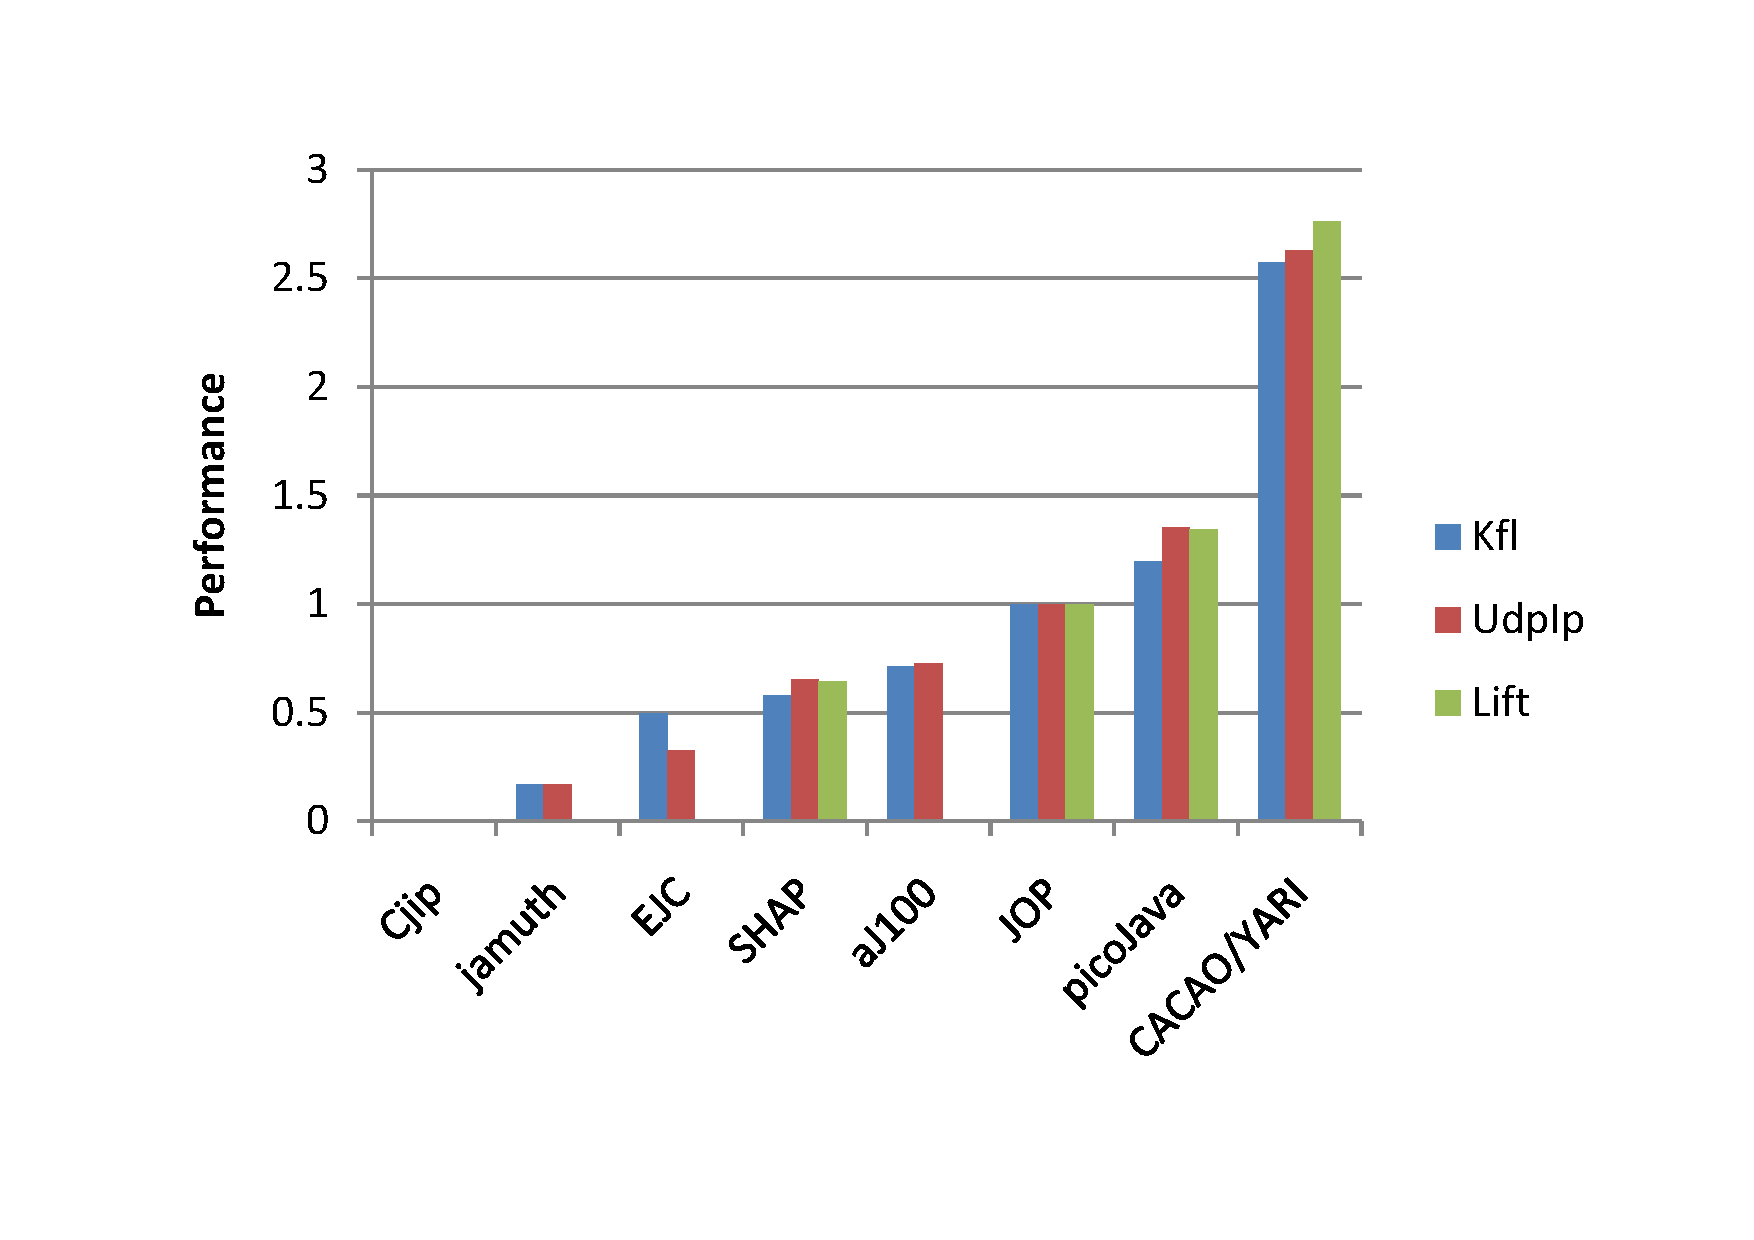
\includegraphics[width=\excelwidth]{results/perf}
    \caption{Performance comparison of different Java systems with
    embedded application benchmarks. The results are scaled to the performance of JOP}
    \label{fig:bench}
\end{figure}

\index{Java processor!aJile} \index{Java processor!Cjip} \index{Java
processor!jamuth} \index{Java processor!SHAP}

Cjip \cite{Cjip} and aJ100 \cite{aJile} are commercial Java
processors, which are implemented in an ASIC and clocked at 80 and
100~Mhz, respectively. Both cores do not cache instructions. The
aj100 contains a 32~KB on-chip stack memory. jamuth
\cite{jamuth:jtres07} and SHAP \cite{shap} are Java processors that
are implemented in an FPGA. jamuth is the commercial version of the
Java processor Komodo \cite{komodo2003}, a research project for
real-time chip multithreading. jamuth is configured with a 4~KB
direct-mapped instruction cache for the measurements. The
architecture of SHAP is based on JOP and enhanced with a hardware
object manager. SHAP also implements the method cache
\cite{shap:mcache}. The benchmark results for SHAP are taken from the
SHAP website.\footnote{\url{http://shap.inf.tu-dresden.de/}, accessed
December, 2008} SHAP is configured with a 2~KB method cache and 2~KB
stack cache.

\index{Java processor!picoJava}

picoJava \cite{pJ1} is a Java processor developed by Sun. picoJava is
no longer produced and the second version (picoJava-II) was available
as open-source Verilog code. Puffitsch implemented picoJava-II in an
FPGA (Altera Cyclone-II) and the performance numbers are obtained
from that implementation \cite{master:puffitsch}. picoJava is
configured with a direct-mapped instruction cache and a 2-way
set-associative data cache. Both caches are 16~KB.

EJC \cite{EJC} is an example of a JIT system on a RISC processor
(32-bit ARM720T at 74~MHz). The ARM720T contains an 8~KB unified
cache. To compare JOP with a JIT based system in exactly the same
hardware we use the research JVM CACAO \cite{cacao} on top of the
MIPS compatible soft-core YARI \cite{cacao:yari}. YARI is configured
with a 4-way set-associative instruction cache and a 4-way
set-associative write-through data cache. Both caches are 8~KB.

The measurements do not provide a clear answer to the question of
whether a time-predictable architecture is slow. JOP is about 40\%
faster than the commercial Java processor aJ100, but picoJava is 30\%
faster than JOP and the JIT/RISC combination (CACAO/YARI) is about
2.7 times faster than JOP. We conclude that a time-predictable
solution will never be as fast in the average case as a solution
optimized for the average case.

%%\subsection{Notes for targets}
%%
%%\subsubsection{JStamp}
%%
%%\begin{verbatim}
%%    aJile project in \usr2\ajile\bench
%%    Sources from JOP target
%%    LowLevel.java from directory aJile
%%    Remove .class in ...\dist\classes
%%    Generate .class with \bat\ajc.bat in source directory
%%        destination is ...\dist\classes
%%        e.g. in ...\src\bench: ajc jbe/DoAll
%%    aJile ChemBuilder (bench.ajp) use COM1 for System.out
%%    Terminal on Serial A, 9600 baud
%%        Did not get the System.out in Charade (but it worked some
%%        time ago)
%%    Charade: Reset, File-Load \usr2\ajile\bench\build.bin
%%\end{verbatim}


\section{Applications}
\label{sec:applications}


Since the start of the development of JOP in late 2000 it has been
successfully deployed in several embedded control and automation
systems. The following section highlights three different industrial
real-time applications that are based on JOP. This section is based
on \cite{jop:app}; the first application is also described in
\cite{jop:wises03}.

Implementation of a processor in an FPGA is a little bit more
expensive than using an ASIC processor. However, additional
application logic, such as a communication controller or an AD
converter, can also be integrated into the FPGA. Integration of the
processor and the surrounding logic in the same reprogrammable chip
is a flexible solution: one can even produce the PCB before all logic
components are developed as the interconnection is programmed on-chip
and not routed on the PCB. For low-volume projects, as those
presented in this section, this flexibility reduces development cost
and therefore outweighs the cost of the FPGA device. It has to be
noted that low-cost FPGAs, that are big enough for JOP, are available
at \$11 for a single unit.

Furthermore, most embedded systems are implemented as distributed
systems and even very small and memory constraint devices need to
communicate. In control applications this communication has to be
performed under real-time constraints. We show in this section
different communication systems that are all based on simple
communication patterns.

\subsection{The Kippfahrleitung}
\label{sec:app:kfl}

The first commercial project where JOP had to prove that a Java
processor is a valuable option for embedded real-time systems was a
distributed motor control system.

In rail cargo, a large amount of time is spent on loading and
unloading of goods wagons. The contact wire above the wagons is the
main obstacle. Balfour Beatty Austria developed and patented a
technical solution, the so-called \emph{Kippfahrleitung}, to tilt up
the contact wire. \figurename~\ref{fig:results:kfl:mast} shows the
construction of the mechanical tilt system driven by an asynchronous
motor (just below the black tube). The little box mounted on the mast
contains the control system. The black cable is the network
interconnection of all control systems. In
\figurename~\ref{fig:results:kfl:mast2} the same mast is shown with
the contact wire tilted up.

\begin{figure}
    \centering
    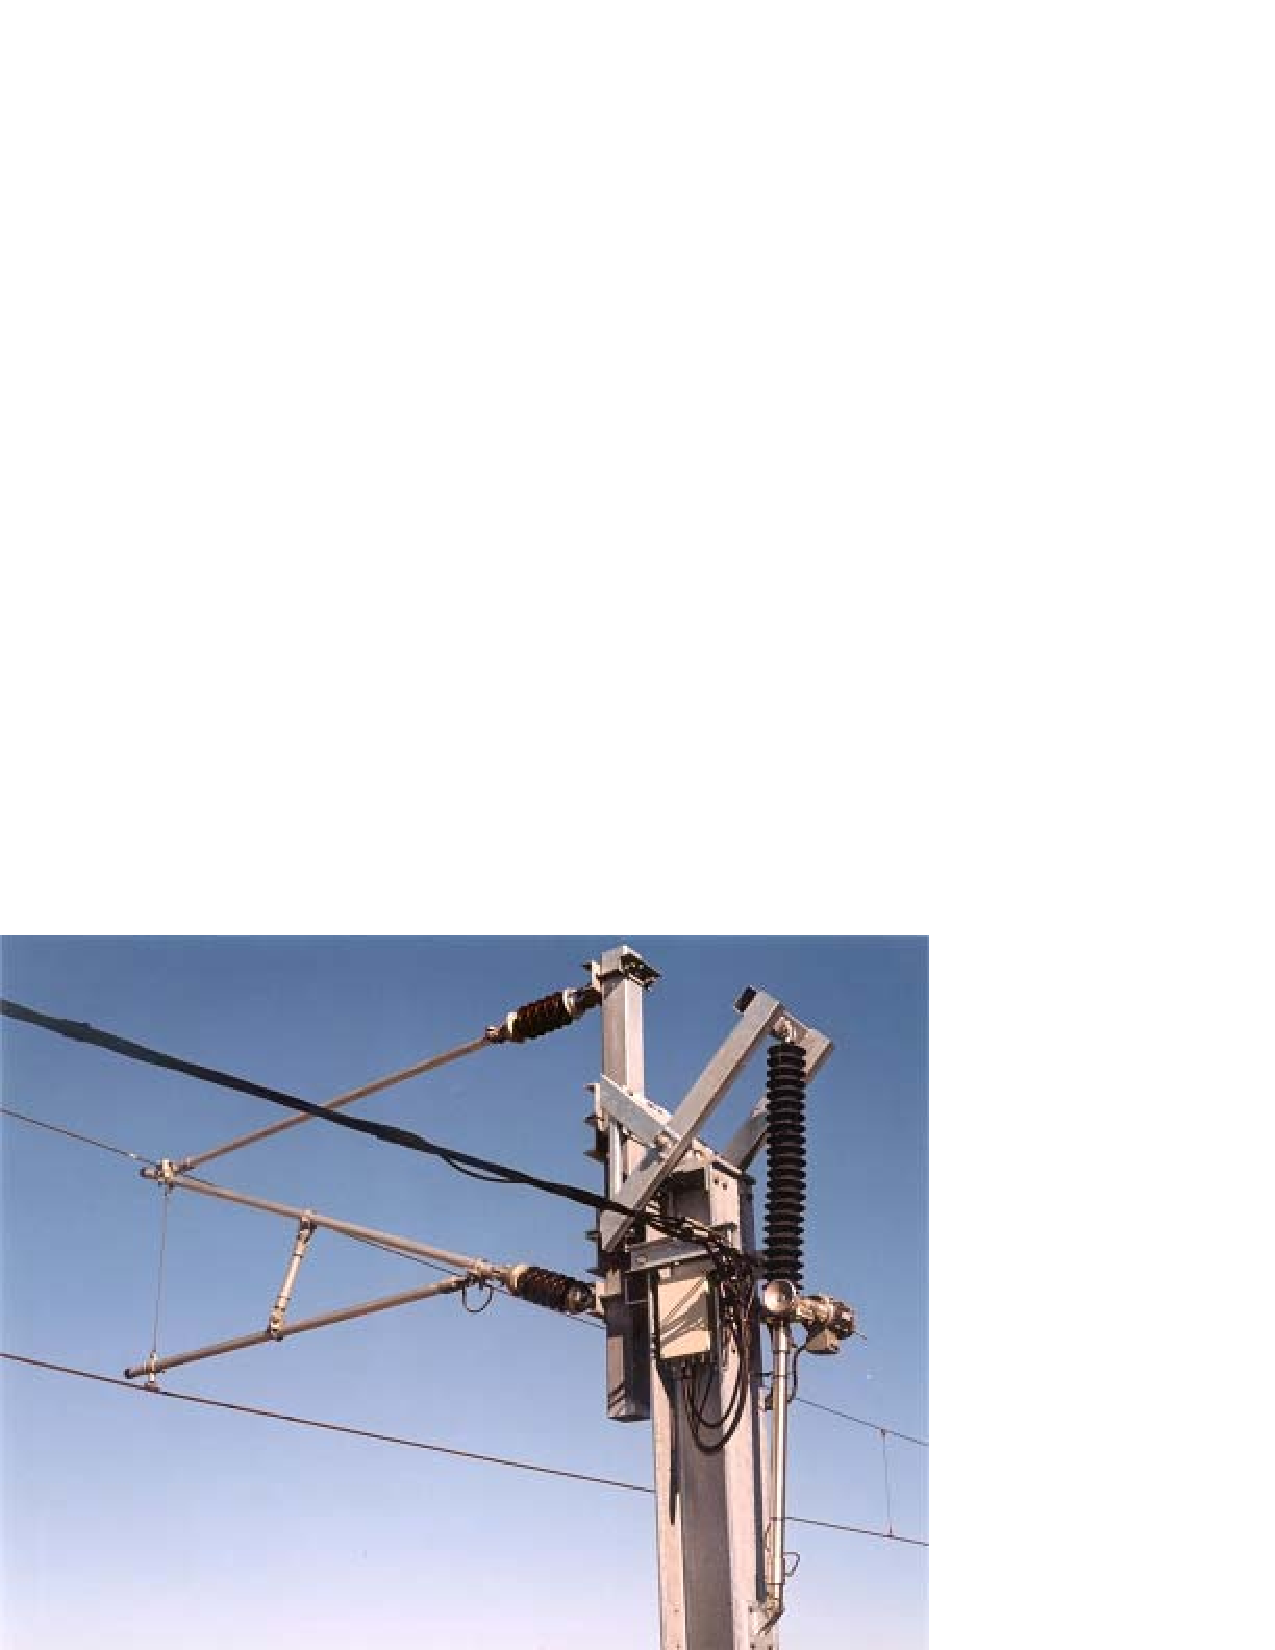
\includegraphics[width=7cm]{results/results_kfl_mast1}
    \caption{A \emph{Kippfahrleitung} mast in down position}
    \label{fig:results:kfl:mast}
\end{figure}


The contact wire is tilted up on a distance of up to one kilometer.
For a maximum distance of 1~km the whole system consists of 12~masts.
Each mast is tilted by an asynchronous motor. However, the individual
motors have to be synchronized so the tilt is performed in a smooth
way. The maximum difference of the position of the contact wire is
10~cm. Therefore, a control algorithm has to slow down the faster
motors.

\begin{figure}
    \centering
    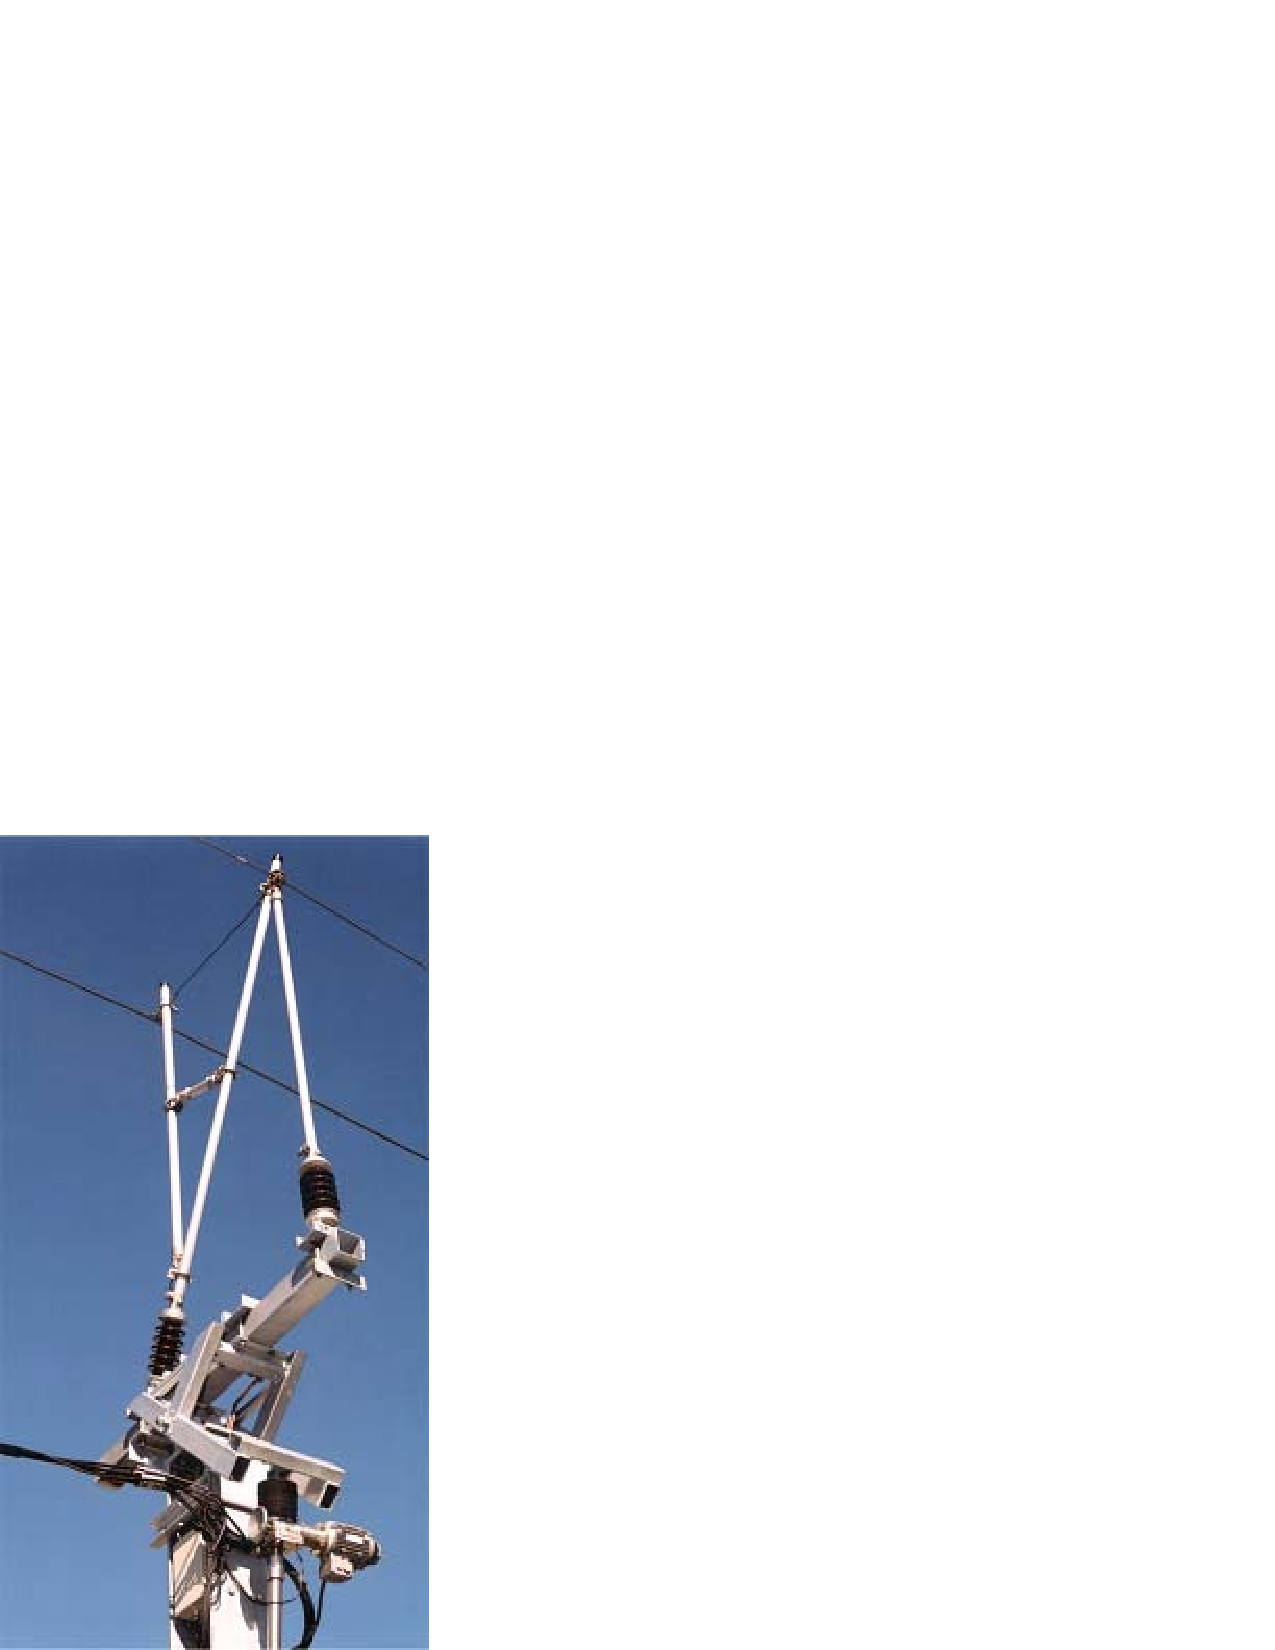
\includegraphics[width=4cm]{results/results_kfl_mast2}
    \caption{The mast in the up position with the tilted contact wire}
    \label{fig:results:kfl:mast2}
\end{figure}

\subsubsection{Hardware}

Each motor is controlled by its own embedded system (as seen in
\figurename~\ref{fig:results:kfl:mast}) by silicon switches. The
system measures the position of the arm with two end sensors and a
revolving sensor. It also supervises the supply voltage and the
amount of current through the motor. Those values are transmitted to
the base station.

The base station, shown in Figure~\ref{fig:results:base}, provides
the user interface for the operator via a simple display and a
keyboard. It is usually located at one end of the line. The base
station acts as master and controls the deviation of individual
positions during the tilt. In technical terms, this is a distributed,
embedded real-time control system, communicating over a shared
network. The communication bus (up to one kilometer) is attached via
an isolated RS485 data interface.

\begin{figure}
    \centering
    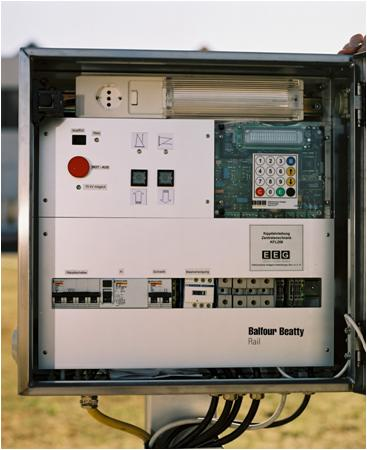
\includegraphics[width=5cm]{results/base}
    \caption{The base station with the operator interface}
    \label{fig:results:base}
\end{figure}


Although this system is not a mass product, there are nevertheless
cost constraints. Even a small FPGA is more expensive than a general
purpose CPU. To compensate for this, additional chips for the memory
and the FPGA configuration were optimized for cost. One standard
128~KB Flash is used to hold FPGA configuration data, the Java
program and a logbook. External main memory is reduced to 128~KB with
an 8-bit data bus. Furthermore, all peripheral components, such as
two UARTS, four sigma delta ADCs, and I/O ports are integrated in the
FPGA.

Five silicon switches in the power line are controlled by the
application program. A wrong setting of the switches due to a
software error could result in a short circuit. Simple logic in the
FPGA (coded in VHDL) can enforce the proper conditions for the
switches. The sigma-delta ADCs are used to measure the temperature of
the silicon switches and the current through the motor.


\subsubsection{Software Architecture}

The main task of the program is to measure the position using the
revolving sensor and to communicate with the base station under
real-time constraints. The conservative style of a cyclic executive
was chosen for the application. At application start all data
structures are allocated and initialized. In the mission phase no
allocation takes place and the cyclic executive loop is entered and
never exited. The simple infinite loop, unblocked at constant time
intervals, is shown in Listing~\ref{lst:results:main}. At the time
the application was developed no static WCET analysis tool for Java
was available. The actual execution time was measured and the maximum
values have been recorded regularly. The loop and communication
periods have been chosen to leave slack fur unexpected execution time
variations. However, the application code and the Java processor are
fully WCET analyzable, as shown later \cite{jop:wcet:jtres06}. The
application is used in Chapter~\ref{chap:wcet} as a test case for the
WCET analysis tool.

No interrupts or direct memory access (DMA) devices that can
influence the execution time are used in the simple system. All
sensors and the communication port are polled in the cyclic
executive.

\begin{lstlisting}[float,caption=The cyclic executive (simplified version),
label=lst:results:main]

private static void forever() {

    for (;;) {
        Msg.loop();
        Triac.loop();
        if (Msg.available) {
            handleMsg();
        } else {
            chkMsgTimeout();
        }
        handleWatchDog();
        Timer.waitForNextInterval();
    }
}
\end{lstlisting}

\subsubsection{Communication}

Communication is based on a master/slave model. Only the base station
(the master) is allowed to send a request to a single mast station.
This station is then required to reply within bounded time. The
master handles timeout and retry. If an irrecoverable error occurs,
the base station switches off the power for all mast stations,
including the power supplies to the motors. This is the safe state of
the whole system.

In a master/slave protocol no media access protocol is needed. In the
case of a failure in the slave that delays a message collision can
occur. The collision is detected by a violation of the message CRC.
Spurious collisions are tolerated due to the retry of the base
station. If the RS485 link is broken and only a subset of the mast
stations reply the base station, the base station switches of the
power supply for the whole system.

On the other hand the mast stations supervise the base station. The
base station is required to send the requests on a regular basis. If
this requirement is violated, each mast station switches off its
motor. The local clocks are not synchronized. The mast stations
measure the time elapsed since the last request from the base station
and locally switch off based on a timeout.

The maximum distance of 1~km determines the maximum baud rate of the
RS485 communication network. The resulting 12 masts on such a long
line determine the number of packets that have to be sent in one
master/slave round. Therefore, the pressure is high on the packet
length. The data is exchanged in small packets of four bytes,
including a one-byte CRC. To simplify the development, commands to
reprogram the Flash in the mast stations and to force a reset are
included. Therefore, it is possible to update the program, or even
change the FPGA configuration, over the network.

\subsection{The SCADA Device TeleAlarm}

TeleAlarm (TAL) is a typical remote terminal unit of a supervisory
control and data acquisition (SCADA) system. It is used by the Lower
Austria's energy provider EVN (electricity, gas, and heating) to
monitor the distribution plant. TeleAlarm also includes output ports
for remote control of gas valves.

\subsubsection{Hardware}

The TAL device consists of a CPU FPGA module and an I/O board. The
FPGA module contains an Altera Cyclone device, 1~MB static memory,
512~KB Flash, and 32~MB NAND Flash. The I/O board contains several
EMC protected digital input and output ports, two 20~mA input ports,
Ethernet connection, and a serial interface. Furthermore, the device
performs loading of a rechargeable battery to survive power down
failures. On power down, an important event for a energy provider, an
alarm is sent. The rechargeable battery is also monitored and the
device switches itself off when the minimal voltage threshold is
reached. This event is sent to the SCADA system before the power is
switched off.

The same hardware is also used for a different project: a lift
control in an automation factory in Turkey. The simple lift control
software is now used as a test case for WCET tool development (see
Chapter~\ref{chap:wcet}).

\subsubsection{Communication}

The communication between the TAL and the main supervisory control
system is performed with a proprietary protocol. On a value change,
the TAL sends the new data to the central system. Furthermore, the
remote units are polled by the central system at a regular base. The
TAL itself also sends the actual state regularly. TAL can communicate
via Internet/Ethernet, a modem, and via SMS to a mobile phone.

EVN uses a mixture of dial-up network and leased lines for the plant
communication. The dial-up modems are hosted by EVN itself. For
safety and security reason there is no connection between the control
network and the office network or the Internet.

\begin{figure}[t]
    \centering
    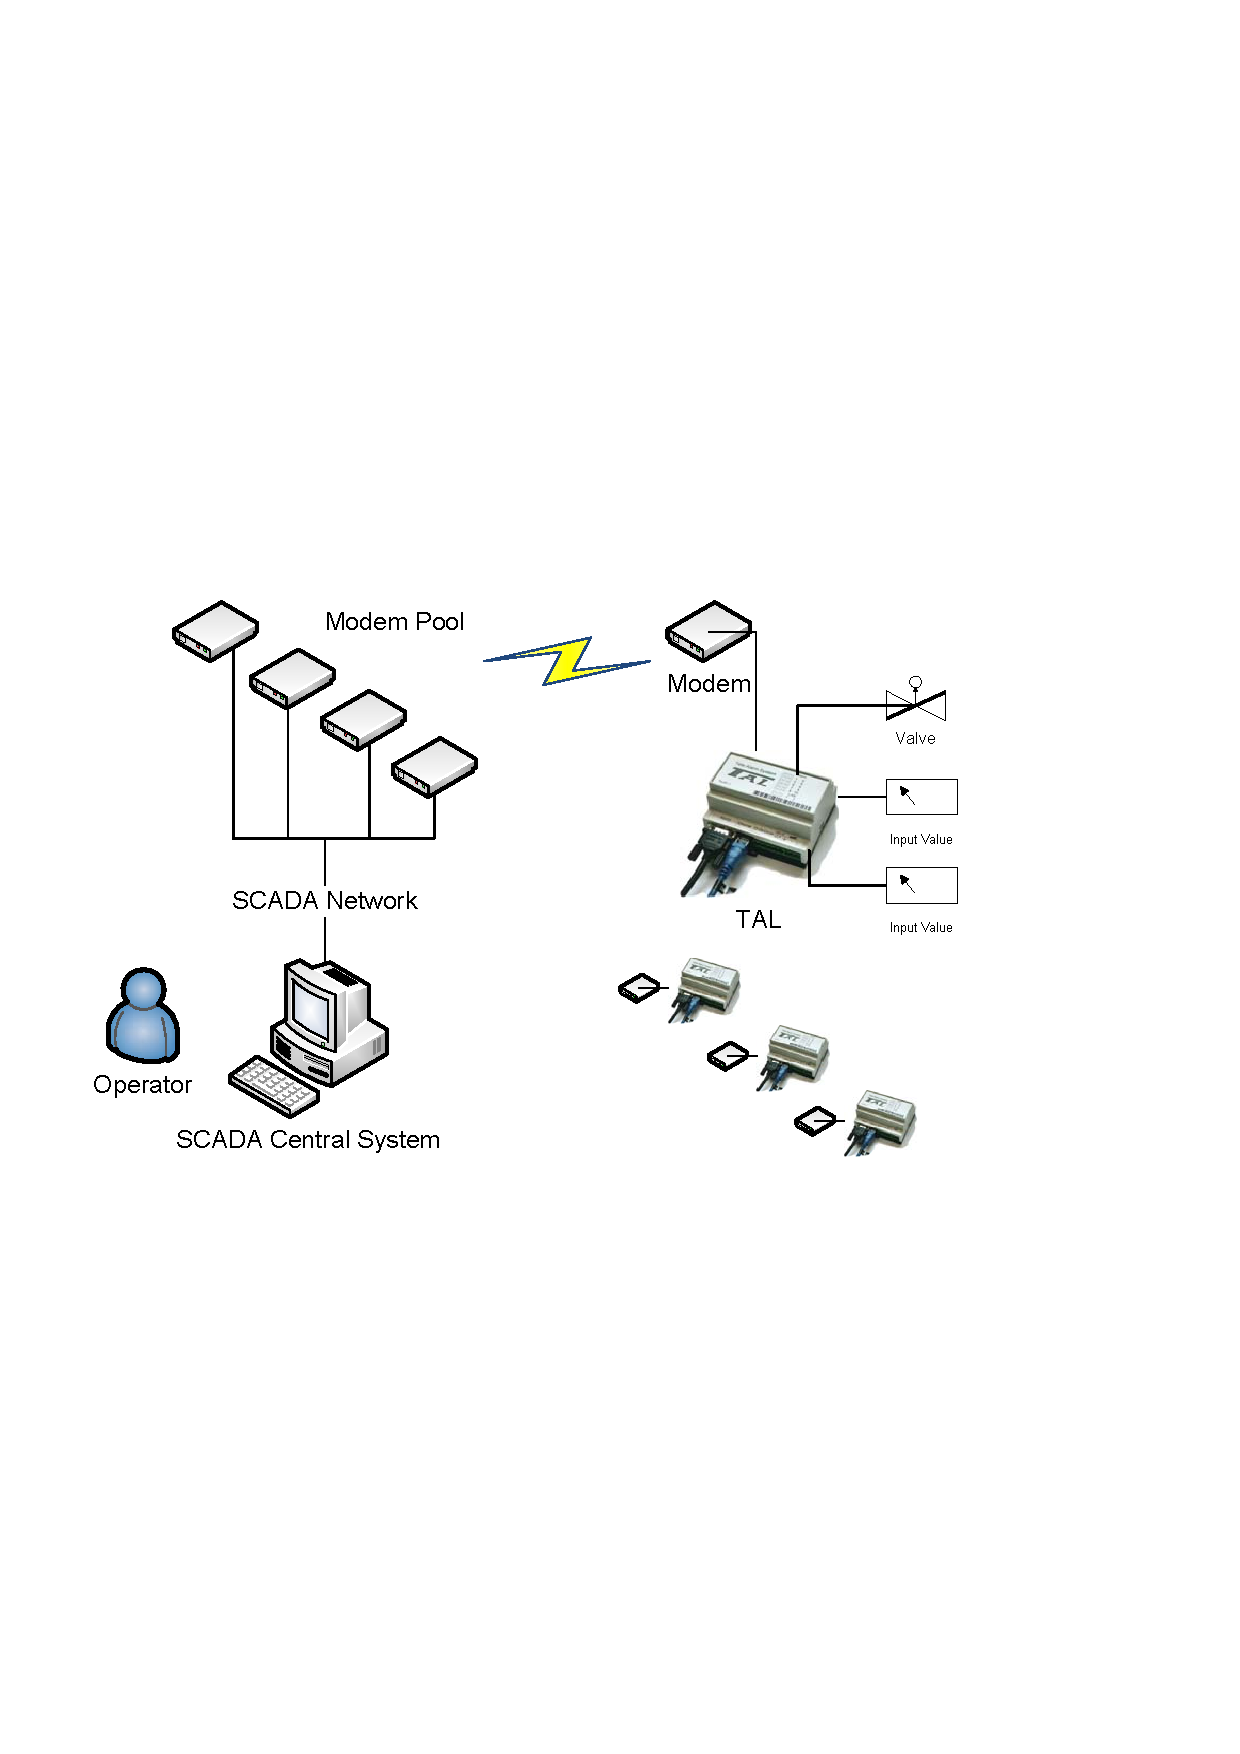
\includegraphics[scale=0.75]{results/tal}
    \caption{EVN SCADA system with the modem pool and TALs as remote terminal units}
    \label{fig:tal}
\end{figure}

\figurename~\ref{fig:tal} shows the SCADA system setup at EVN.
Several TALs are connected via modems to the central modem pool. The
modem pool itself is connected to the central server. It has to be
noted that there are many more TALs in the field than modems in the
pool. The communication is usually very short (several seconds) and
performed on demand and on a long regular interval. Not shown in the
figure are additional SCADA stations and other remote terminal units
from other manufacturers.

\subsection{Support for Single Track Railway Control}

Another application of JOP is in a communication device with soft
real-time properties -- Austrian Railways' (\"OBB) new support system
for single-track lines. The system helps the superintendent at the
railway station to keep track of all trains on the track. He can
submit commands to the engine drivers of the individual trains.
Furthermore, the device checks the current position of the train and
generates an alarm when the train enters a track segment without a
clearance.

At the central station all track segments are administered and
controlled. When a train enters a non-allowed segment all trains
nearby are warned automatically. This warning generates an alarm at
the locomotive and the engine driver has to perform an emergency
stop.

\figurename~\ref{fig:zlb} gives an overview of the system. The
display and command terminal at the railway station is connected to
the Intranet of the railway company. On the right side of the figure
a picture of the terminal that is connected to the Internet via GPRS
and to a GPS receiver is shown. Each locomotive that enters the track
is equipped with either one or two of those terminals.

\begin{figure}
    \centering
    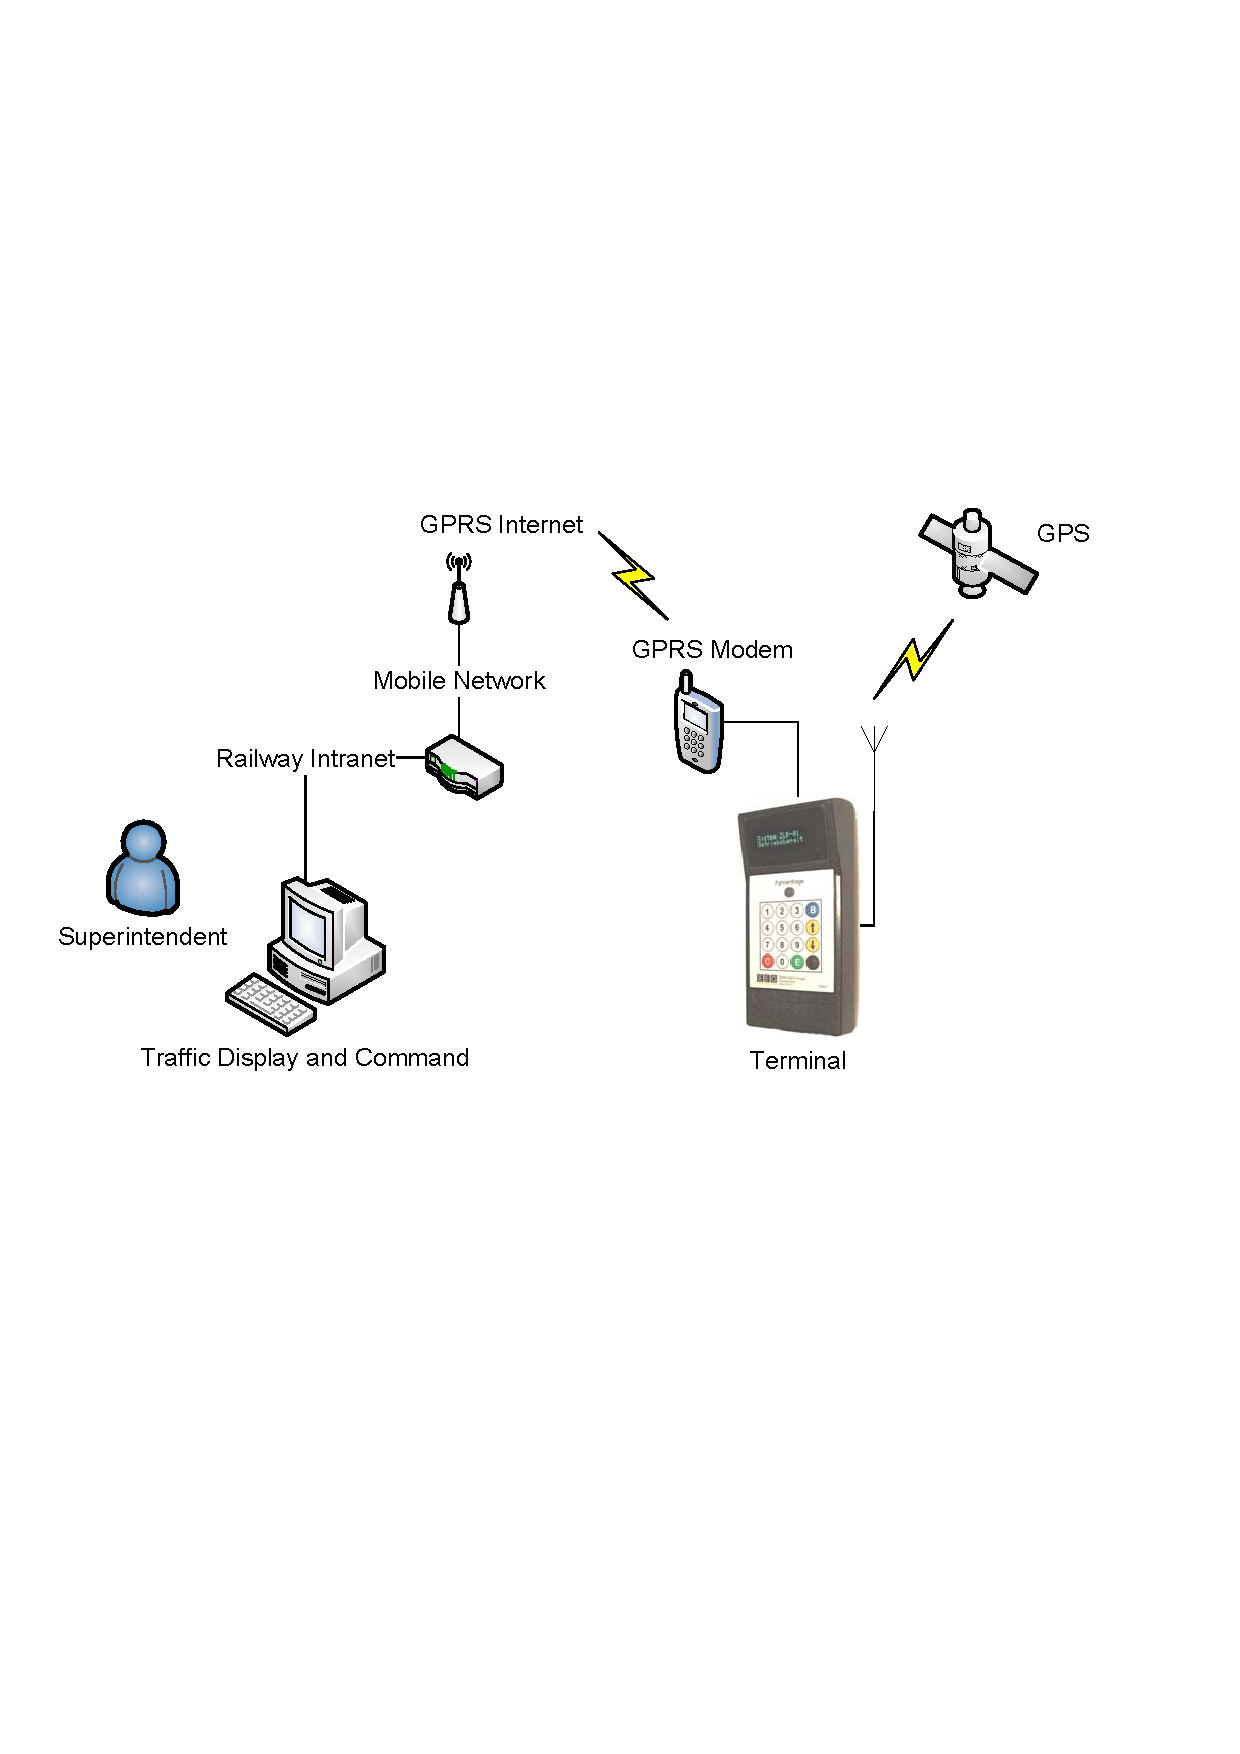
\includegraphics[scale=0.75]{results/zlb}
    \caption{Support system for single track railway control for the Austrian railway company}
    \label{fig:zlb}
\end{figure}

It has to be noted that this system is not a safety-critical system.
The communication over a public mobile phone network is not reliable
and the system is not certified for safety. The intension is just to
\emph{support} the superintendent and the engine drivers.

\subsubsection{Hardware}

Each locomotive is equipped with a GPS receiver, a GPRS modem, and
the communication device (terminal). The terminal is a custom made
device. The FPGA module is the same as in TAL, only the I/O board is
adapted for this application. The I/O board contains several serial
line interfaces for the GPS receiver, the GPRS modem, debug and
download, and display connection. Auxiliary I/O ports connected to
relays are reserved for future use. A possible extension is to stop
the train automatically.

\subsubsection{Communication}

The current position of the train is measured with GPS and the
current track segment is calculated. The number of this segment is
regularly sent to the central station. To increase the accuracy of
the position, differential GPS correction data is transmitted to the
terminal. The differential GPS data is generated by a ground base
reference located at the central station.

The exchange of positions, commands, and alarm messages is performed
via a public mobile phone network (via GPRS). The connection is
secured via a virtual private network that is routed by the mobile
network provider to the railway company's Intranet. The application
protocol is command/response and uses UDP/IP as transport layer. Both
systems (the central server and the terminal) can initiate a command.
The system that sends the command is responsible for retries when no
response arrives. The deadline for the communication of important
messages is in the range of several seconds. After several
non-successful retries the operator is informed about the
communication error. He is than in charge to perform the necessary
actions.

Besides the application specific protocol a TFTP server is
implemented in the terminal. It is used to update the track data for
the position detection and to upload a new version of the software.
The flexibility of the FPGA and an Internet connection to the
embedded system allows to upgrade the software and even the processor
in the field.


\subsection{Communication and Common Design Patterns} \label{sec:comm}

Although we described embedded systems from quite different
application domains we have been facing similar challenges. All
systems are distributed systems and therefore need to communicate.
Furthermore, they are real-time systems (at least with soft
deadlines) and need to trust the communication and perform regular
checks. The issues in the design of embedded real-time systems are
quite similar in the three described projects. We found that several
design patterns are used over and over and describe three of them in
this section.


\subsubsection{Master/Slave Designs}

Developing safe embedded systems is an exercise in reducing
complexity. One paradigm to simplify embedded software development is
the master/slave pattern. Usually a single master is responsible to
initiate commands to the slaves. The single master is also
responsible to handle reliable communication. The master/slave
pattern also fits very well with the command/response pattern for the
communication.

\subsubsection{Dealing with Communication Errors}

Communication is not per se reliable. The RS485 link at the
Kippfahrleitung operates in a rough environment and electromagnetic
influences can lead to packet loss. The TAL system can suffer from
broken phone lines. The single track control system operates on a
public mobile phone network -- a network without any guarantees for
the GPRS data traffic. Therefore, we have to find solutions to
operate in a safe and controlled manner the distributed system
despite the chance of communication errors and failures.

Reliable communication is usually provided by the transport layer,
TCP/IP in the case of the Internet. However, the timeouts in TCP/IP
are way longer than the communication deadlines within control
systems. The approach in all three presented projects is to use a
datagram oriented protocol and perform the timeout and retransmission
at the application level. To simplify the timeout handling a simple
command and response pattern is used. One partner sends a command and
expects the response within a specific time bound. The command
initiator is responsible for retransmission after the timeout. The
response partner just needs to reply to the command and does not need
to remember the state of the communication. After several timeouts
the communication error is handled by an upper layer. Either the
operator is informed (in the SCADA and the railway control system) or
the whole system is brought into a safe state (in the motor control
project).

Communication errors are either transient or longer lasting.
Transient communication errors are lost packets due to network
overload or external electromagnetic influences. In a
command/response system the lost packets (either the command or the
response) is detected by a timeout on the response. A simple
retransmission of the command can correct those transient errors.

A longer network failure, e.g.\ caused by a wire break, can be
detected by too many transmission retries. In such a case the system
has to enter some form of safe state. Either the power is switched
off or a human operator has to be informed. The individual timeout
values and the number of retries depend, similar to thread periods,
on the controlled environment. In the Kippfahrleitung the maximum
timeout is in the millisecond range, whereas in the SCADA system the
timeout is several minutes.

\subsubsection{Software Update}

Correction of implementation bugs during development can be very
costly when physical access to the embedded system is necessary for a
software update. Furthermore, a system is usually never really
finished. When the system is in use the customer often finds new ways
to enhance the system or requests additional features.

Therefore, an important feature of a networked embedded system is a
software and parameter update in the field. In the first project the
software update is performed via a home-made protocol. The other
projects use the Internet protocol to some extent and therefore TFTP
is a natural choice. TFTP is a very simple protocol that can be
implemented within about 100 lines of code. It is applicable even in
very small and resource constraint embedded devices.

\subsection{Discussion} \label{sec:lessions}

Writing embedded control software in Java is still not very common
due to the lack of small and efficient implementations of the JVM.
Our Java processor JOP is a solution for some embedded systems.

Using Java as the implementation language was a pleasure during
programming and debugging. We did not waste many hours to hunt for
pointer related bugs. The stricter (compared to C) type system of
Java also catches many more programming errors at compile time.
However, when using Java in a small embedded system one should not
expect that a full blown Java library is available. Almost all of the
code had to be written without library support. Embedded C
programmers are aware of that fact, but Java programmers are new in
the embedded domain and have to learn the difference between a PC and
a 1~MB memory embedded system.

Up to date FPGAs in embedded control systems are only used for
auxiliary functions or to implement high-performance DPS algorithm
directly in hardware. Using the FPGA as the main processor is still
not very common. However, combining the main processor with some
peripheral devices in the same chip can simplify the PCB layout and
also reduce the production cost. Furthermore, a field-reprogrammable
hardware device offers a great deal of flexibility: When some part of
the software becomes the bottleneck, an implementation of that
function in hardware can be a solution. Leaving some headroom in the
logic resources can extend the lifetime of the product.

For a prototype, JOP has been attached to a time-triggered
network-on-chip \cite{jop:ttnoc}. It would be an interesting exercise
to implement a JOP based node in a time-triggered distributed system
as proposed by \cite{journals/pieee/KopetzB03}. The combination of a
real-time Java processor and a real-time network can ensure real-time
characteristics for the whole system.


\section{Summary}

In this chapter, we presented an evaluation of JOP. We have seen
that JOP is the smallest hardware realization of the JVM available
to date. Due to the efficient implementation of the stack
architecture, JOP is also smaller than a \emph{comparable} RISC
processor in an FPGA. Implemented in an FPGA, JOP has the highest
clock frequency of all known Java processors.

We compared JOP against several embedded Java systems. JOP is about
40\% faster than the commercial Java processor aJ100, but picoJava
and a JIT/RISC combination are faster than JOP. These results show
that a time-predictable architecture does not need to be slow, but
will never be as fast as an architecture optimized for average case
performance.

Furthermore, we have presented three industrial applications
implemented in Java on an embedded, real-time Java processor. All
projects included custom designed hardware (digital functions) and
the central computation unit implemented in a single FPGA. The
applications are written in pure Java without the need for native
methods in C. Java proved to be a productive implementation language
for embedded systems. Usage of JOP in four real-world applications
showed that the processor is mature enough to be used in commercial
projects.
